\documentclass[12pt,titlepage,final]{article}
\usepackage{graphicx}
\usepackage{mathtools}
\begin{document}

\title{\textsc{Modern Interferometry Lab}}
\author{Anthony Ford, Alex Garcia, Rossina Miller}
\date{November 30, 2011}
\maketitle

\clearpage

\begin{abstract}
The objective of this experiment was to assemble a Michelson Interferometer,
experiment with different ways of viewing the interference patterns, and explore
methods of measuring the alignment and achieving optimum alignment. We were able
to properly construct and align our Michelson Interferometer, achieving a
visibility of \emph{***BLAH***}.
\end{abstract}



\section{Theory}

\section{Theory}

The purpose of this experiment is to see how an interferometer works. The
Michelson interferometer is the design that will be used for the experiment. A
Michelson interferometer is a simple interferometer that is used to make very
small and precise measurements, in fact the Michelson interferometer is the
layout used in LIGO\@. A Michelson interferometer works by having a laser shoot
down a path into a beam splitter that splits the laser beam into two seperate
paths. At the end of each path there is a mirror that will reflect the laser
back toward the beam splitter which then combines the two beams. After the
recombination the lasers will be either in or out of phase, due to the
superposition principle. The superposition principle basically says that when
two waves pass through the same point in space their amplitudes will combine;
this causes the net amplitude to add or subtract, known as constructive and
destructive interference respectively. Constructive interference happens if the
waves are in phase while destructive interference happens when the waves are out
of phase.

\begin{figure}[ht!]
\centering
%Caption: Two waves in phase and the next is two waves 180 degress out of phase
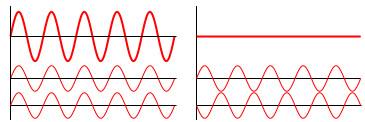
\includegraphics[width=4 in]{Interference_of_two_waves}
\caption{Two waves in phase and the next is two waves 180 degrees out of phase}
\end{figure}

In this experiment the only way that the phase will change will be due to the distance between the mirrors and the beam splitter. The phase difference,$\Delta \phi$, is calculated by 
	\begin{align}
		\nonumber \Delta \phi &=\frac{2\pi}{\lambda} \Delta p
	\end{align}
with $\Delta p$ being the difference in the paths and $\lambda$ being the wavelength of the laser being used. From there we can then say that 
	\begin{align}
		\nonumber \Delta p &=\sum(n_2 d_2)-\sum(n_1 d_1) \\
		\nonumber		&=n_2 d_2 - n_1 d_1
	\end{align} 
where $d$ is the distance from the beam splitter to the cube and $n$ is index of refraction of the medium the beam is traveling through. For this experiment the medium's are the same, they are both traveling through air, so then $n_1=n_2$ which results in
	\begin{align}
		\nonumber \Delta p &= n_2 d_2 - n_1 d_1 \\
		\nonumber 	&= n(d_2 - d_1) \\
		\nonumber \Delta \phi &=\frac{2\pi n}{\lambda} (d_2 - d_1)
	\end{align}

The change in phase will then affect the intensity of the beam, causing fringes to appear. These fringes will be red and black rings on a screen or piece of paper behind the lens. The black rings signify a destructive interference while the red rings are due to the constructive interference. 

Using a photodiode to get the fringes to appear on an oscilloscope it is then possible to get the voltage required to move from one fringe to another. Using this information with the properties of the piezo stack it is possible to get the wavelength of the laser. 



%The purpose of this experiment is to measure\ldots

%Start with the motivation (or reason) for the experiment. Follow this with the theory behind the experiment. Give a brief presentation, in your own words, of the essential ideas behind the experiment. Include only the most important formulas (explaining the meaning of any symbols used). Do not give any derivations unless they are original. The purpose is just to establish the context of the experiment and state, for reference, the relations you will be using in analyzing your data. (The proverbial interested reader should be able to look up details elsewhere on the basis of your outline.) One paragraph, in good English, should suffice.

\section{Description}

We used a Michelson interferometer and\ldots

%Succinctly describe, in your own words, the apparatus used and the procedures followed to get your results. It is best to do this without reference to the lab manual. Relying on your own memory is more authentic and provides practice for your powers of observation. Tell what you did so that someone else could duplicate it from your description. This is an instructive exercise, for your benefit, in attending to and understanding facts in a scientific manner and to give you practice in describing them intelligibly. Think of your reader as an intelligent student who has not done the experiment. You should demonstrate clearly that you know and understand what you did and can articulate it simply.Often the simplest and clearest way to explain something is to give a schematic drawing. This means a drawing without the details that are not essential to the point you are trying to communicate. For example, in discussing the motion of a car, is more appropriate than, because the essence is that something is moving from one place to another and the details of the object moving are irrelevant. It is important to gain the skill of realizing and illustrating the essence of a situation.

\section{Measurements}
%Write down, preferably in tabular form, every measurement you took and what was taken into account in the following results section.


\begin{tabular*}{1.16\textwidth}{| @{\hspace{.5cm}}r | @{\hspace{.5cm}}r | @{\hspace{.5cm}}r | @{\hspace{.5cm}}r 
				|@{\hspace{.5cm}}r  | @{\hspace{.5cm}}r | @{\hspace{.5cm}}r | @{\hspace{.5cm}}r || @{\hspace{.5cm}}r |}
	\hline
	$\Delta V_1$ & $\Delta V_2$ & $\Delta V_3$ & $\Delta V_4$ & $\Delta V_5$ & $\Delta V_6$ & 
	$\Delta V_7$ & $\Delta V_8$ & Avg $\Delta V$ \\
    \hline 
	6.0 V & 6.4 V & 5.4 V & 5.6 V & 6.6 V & 7.2 V & 3.6 V & 6.0 V &     5.85 V\\
    \hline
    6.2 V & 5.8 V & 6.4 V & 5.6 V & 7.2 V & 5.6 V & 7.0 V & 5.4 V &     6.15 V\\
    \hline

\end{tabular*}

\section{Results/Analysis}
%Lay out the calculations that you are doing, never present results without explaining how you derived them. For your own benefit (and for the instructor's sanity): BE NEAT! 
%When you present data ALWAYS include an estimate of the error and show how the error analysis was performed. Clearly state the results you obtain. Results should be presented in an organized form, such as in tables, charts and graphs, and stated in correct SI units. When appropriate, experimental results should be compared to theoretical predictions and calculations. Include the percent error when appropriate. Don't use terms such as "fairly close" and "pretty good;" give explicit quantitative deviations from the expected result. Evaluate whether these deviations fall within your expected errors and state possible explanations for unusual deviations.

\section{Summary}
%Summarize, in a paragraph or two, what you conclude from the results of your experiment and whether they are what you expected them to be. Include brief answers to the specific questions asked in the lab instructions.

\section{Remarks}
%Please critique the experiment as presented in the lab manual. Could the lab be done in a better way? Do you have some other or original method for obtaining the same results? Your suggestions are encouraged and are used to improve the lab manual.

  
\end{document}
